\documentclass[10pt, a4paper]{beamer}
%\documentclass{article}

%Metadaten
\title{Machine Vision with Arduino Portenta H7}

\subtitle{Getting Started With the Portenta Vision Shield Camera - Save Images}
%\institution{University of Applied Science Hochschule Emden/Leer}
\author{Vijay Singh}
%\date{\today}
\date{\today}

% siehe hesader.tex Zeile 10-16 zum Aktivieren der Notes
% Kommentare stehen in \notes{} und können im 2-screen-mode genutzt werden
%%%%%%
%
% $Autor: Wings $
% $Datum: 2020-01-18 11:15:45Z $
% $Pfad: githubtemplate/Template/Presentations/Template/slides/header.tex $
% $Version: 4620 $
%
%
% !TeX encoding = utf8
% !TeX root = Rename
%
%%%%%%


%Packages
\usepackage[utf8]{inputenc} %Für Umlaute, da BibLaTeX
\usepackage[german]{babel}
\usepackage{amsmath}
\usepackage{amsfonts}
\usepackage{amssymb}
\usepackage{colortbl}
\usepackage{cancel} %'\cancel{}', '\bcancel{}' und '\xcancel{}'

%%%%%%%%%2-Screen%%%%%%%%%%%%%%%%%%%%%%%%%%%%%%%%%%%%%%%%%%%%
\usepackage{pgfpages} 
%%%%Kommentiert für Beamer
%%%%Aktiv für Notes
%\setbeameroption{show notes on second screen=bottom}
%\setbeameroption{second mode text on second screen=bottom}
%%%%%%%%%%%%%%%%%%%%%%%%%%%%%%%%%%%%%%%%%%%%%%%%%%%%%%%%%%%%%

%Für Grafiken
\usepackage{tikz}
\usetikzlibrary{mindmap}
\usepackage{gnuplottex}
\usepackage{pgf}
\usepackage{colortbl} 
\usetikzlibrary{calc}
\usetikzlibrary{shapes,arrows} %Für Flowchart
\usetikzlibrary{shapes.geometric} %Für Flowchart
\usepackage{scalefnt}
\usetikzlibrary{decorations.markings} %Für => pfeile
\usetikzlibrary{calc,patterns,decorations.pathmorphing,decorations.markings}
%Für urls in Quellen
\usepackage{url}
%Für Diagramme (autotools)
%\usepackage{graphicx}
%\usepackage{graphviz}

%\usepackage[
%  backend=biber,
%  style=alphabetic,
%  sorting=ynt
%]{biblatex}

\usepackage[natbib=true,style=alphabetic,backend=bibtex,useprefix=true]{biblatex}

%Formatierungen
\mode<presentation>
\setbeamertemplate{headline} 
{%
\begin{beamercolorbox}[rounded=true, center]{bgcolor}
\begin{columns}[T]
\begin{column}{9cm}
{\color{gray}\begin{tiny}Hochschule Emden/Leer\end{tiny}} \\ 
{\color{gray}\begin{tiny}Department of Electrical and Computer Engineering\end{tiny}} \\ 
{\color{gray}\begin{tiny}Industrial Informatics\end{tiny}} \\
%{\color{gray}\begin{tiny}Innovationsforum MSR\end{tiny}}
\end{column}
\begin{column}{2cm}

\includegraphics[scale=0.25]{img/technik.jpg}
\end{column}
\end{columns}
\end{beamercolorbox}
 }
\insertsectionhead
\insertsubsectionhead
\usetheme{default}
\useinnertheme[shadow=true]{rounded}
\usebackgroundtemplate
{%
      \rule{0pt}{\paperheight}%
      \hspace*{\paperwidth}%
      \makebox[0pt][r]{
\includegraphics[width=\paperwidth]{img/hintergrund2.png}}
 }

\definecolor{HSELhellblau}{RGB}{138,198,203}
\definecolor{HSELblau}{RGB}{0,59,95}
\usecolortheme[named=HSELblau]{structure}
 \newcommand{\topline}{%
  \tikz[remember picture,overlay] {%
    \draw[HSELhellblau] ([yshift=-0.9cm]current page.north west)
             -- ([yshift=-0.9cm,xshift=\paperwidth]current page.north west);}}
\setbeamertemplate{section}[numbered]


\newcommand{\STANDARD}[2]
{
  \mode<presentation>%
  {%
     \begin{frame}[allowframebreaks]{#1} #2 \end{frame}
  }%
  \mode<article>
  {
    \fcolorbox{AliceBlue}%{Bisque} %{BlanchedAlmond}
    {LightGrey} %{Beige}   %{AliceBlue}
    {
      \begin{minipage}{\textwidth}{\bf #1} #2  \end{minipage}
      
      
    }%
    
    \medskip
    \hrulefill
  }
}

\newcommand{\MYNOTE}[1]
{
  \mode<presentation>%
  {%
     %\note{#1}
     \only<article>{#1}
  }%
  \mode<article>
  {
    #1
  }
}

% ------------
% sectionframe
% ------------
%
% #1  Der Name der section.
%
\newcommand{\sectionframe}[1]%
{%
	\begin{frame}
		\Huge
		\begin{center}
			#1 
		\end{center}
	\end{frame}%
}

\newcommand{\Mysection}[1]%
{%
  \section{#1}%
  
  \sectionframe{#1}%
}

\usepackage{listings}

% Farben für Syntax-Highlighting
\definecolor{dkgreen}{rgb}{0,.6,0}
\definecolor{dkblue}{rgb}{0.655,0.113,.364}
\definecolor{dkyellow}{cmyk}{0,0,.8,.3}

\definecolor{parameterc}{rgb}{.4,0,.6}
\definecolor{typec}{rgb}{0,0.525,.702}
\definecolor{stringc}{rgb}{0,.5019,.5019}
\definecolor{keywordc}{rgb}{.6549, .1137, .3647}
\definecolor{commentc}{rgb}{.5882, .5960, .5882}
\definecolor{textc}{rgb}{.2,.2,.2}

\lstdefinestyle{all}{
	alsoletter={-},
	frame=single, 	% top,frame=bottom,
	numbers=none,
	numberstyle=\tiny\color{textc},
	basicstyle=\linespread{0.9}\ttfamily\footnotesize\color{textc},
	tabsize=4,
	showstringspaces=false,
	captionpos=t,
	rulecolor=\color{lightgray!40},
	keywordstyle=\color{keywordc},
	stringstyle=\color{stringc},
	commentstyle=\color{commentc},
	breaklines=true,
	escapechar="!",
	postbreak=\mbox{\textcolor{green}{$\hookrightarrow$}\space},
}

\lstdefinestyle{bashstyle}{
	style=all,
	keywords=[2]{-y, --no-install-recommends, --allow-change-held-packages, --allow-downgrades, --fetch-keys, -n, --version, --params, -c, -i, -O, --upgrade, --no-cache-dir, --extra-index-url, --show, -s, -m},
	keywordstyle=[2]\color{parameterc},
	morekeywords = {ln,choco,pip,pip3,apt,apt-key,apt-get,apt-mark,add-apt-repository,wget,mktemp,dpkg,dpkg-query,echo,>>,rm,tegrastats, systemctl},
	deletekeywords={local,LOCAL},
}

\lstdefinestyle{pythonstyle}{
	style=all,
	morekeywords={as},
	keywords=[2]{True, False, None},
	keywordstyle=[2]\color{typec},
	alsoletter={_},
	keywords=[3]{max_workspace_size_bytes, precision_mode, maximum_cached_engines, use_calibration, optimizer, loss, input_shape, from_logits, metrics, batch_size, epochs, validation_data, activation, use_calibration, filters, kernel_size, pool_size, units},
	keywordstyle=[3]\color{parameterc},
	deletekeywords={compile,COMPILE},
}

\lstdefinestyle{inlinestyle}{
	style=all,
	breaklines        = true,
	breakatwhitespace = true,
	breakindent       = 2ex,
	escapechar        = *,
	numbers           = left,
	postbreak=,
}
\lstdefinelanguage{MyBash} {
	language = Bash,
	style=bashstyle,
}

\lstdefinelanguage{MyPython} {
	language = Python,
	style=pythonstyle,
}


\definecolor{PythonColor}{rgb}{0,0.5,1.}
\newcommand{\PYTHON}[1]{\textcolor{PythonColor}{\texttt{#1}}}
\definecolor{PythonColorHighLite}{rgb}{0.5,0,1.}
\newcommand{\PYTHONHL}[1]{\textcolor{PythonColorHighLite}{\texttt{#1}}}
\definecolor{MapleColor}{rgb}{1,0,0}
\newcommand{\MapleCommand}[1]{\textcolor{MapleColor}{\texttt{#1}}}
\definecolor{ShellColor}{rgb}{0,1,1.}
\newcommand{\SHELL}[1]{\textcolor{ShellColor}{\texttt{#1}}}
\definecolor{FileColor}{rgb}{1,0,1.}
\newcommand{\FILE}[1]{\textcolor{FileColor}{\texttt{#1}}}

%\addbibresource{Documents/MyLiterature.bib} %Import the bibliography file

\usepackage{listings}
\usepackage{xcolor}

\lstset{
	basicstyle=\ttfamily\small,
	keywordstyle=\color{blue},
	commentstyle=\color{gray},
	stringstyle=\color{red},
	numberstyle=\tiny\color{gray},
	stepnumber=1,
	numbersep=10pt,
	backgroundcolor=\color{white},
	showspaces=false,
	showstringspaces=false,
	breaklines=true,
	frame=single,
	tabsize=2,
	captionpos=b
}

\begin{document}
	
	
\setbeamercolor{bgcolor}{fg=black,bg=white}
\selectlanguage{german}
\setbeamertemplate{footline}{%
\vspace*{-.1cm}\hspace*{.5cm}
\scriptsize{%
%%\hspace*{1pt}\insertauthor
%%\inserttitle
\hspace{325pt}\insertframenumber/\inserttotalframenumber}
}

\STANDARD{}
{
  \titlepage
}

\MYNOTE
{
  \ldots
}



\STANDARD{}
{
\tableofcontents[hideallsubsections]
}

\MYNOTE
{
  \ldots
}

\setbeamercovered{transparent}
	
	\section{Overview}
	\begin{frame}
		\frametitle{Introduction}
		
		\begin{block}{}
			This tutorial shows you how to capture a frame from the \textbf{Portenta Vision Shield} Camera module and save the output as a bitmap image. It will allow you to see the output directly on your computer without using any third party tool. ~\ref{arduinoVisionShield:2024}
		\end{block}
		
		
		\begin{block}{Objectives}
			\begin{itemize}
				\item Capturing the frames from the camera
				\item Make the bitmap binary file with the correct settings.
				\item Save the bitmap on a SD Card and PC.
				\item Visualize the captured image on your computer.
			\end{itemize}
		\end{block}
		
		\begin{block}{Importance}
			Real-time object detection has applications in surveillance, industrial automation, robotics, and IoT, among others.
		\end{block}
		
	\end{frame}
	
	\section{Components}
	\begin{frame}
		
	
		\frametitle{Required Hardware and Software}
		
		\begin{block}{Description}
			The project involves the following components:
			\begin{itemize}
				\item \textbf{Arduino Portenta H7:} The core microcontroller unit providing processing power and resources for boarding different shields.
				\item \textbf{Portenta Vision Shield:} An accessory for the Portenta H7, equipped with a camera module and display for image capture and processing.
				\item \textbf{USB-C cable:} A pre-trained model deployed on the Portenta H7 for object detection tasks.
				\item \textbf{Micro SD card:} A arduino software to capture the image data by the onboard camera.
				\item \textbf{Arduino IDE:} A processing software helps to visualize the data
			\end{itemize}
		\end{block}
		
	\end{frame}
	
	\begin{frame}
		\frametitle{Figures}
		
		\begin{columns}
			\column{0.5\textwidth}
			\centering
			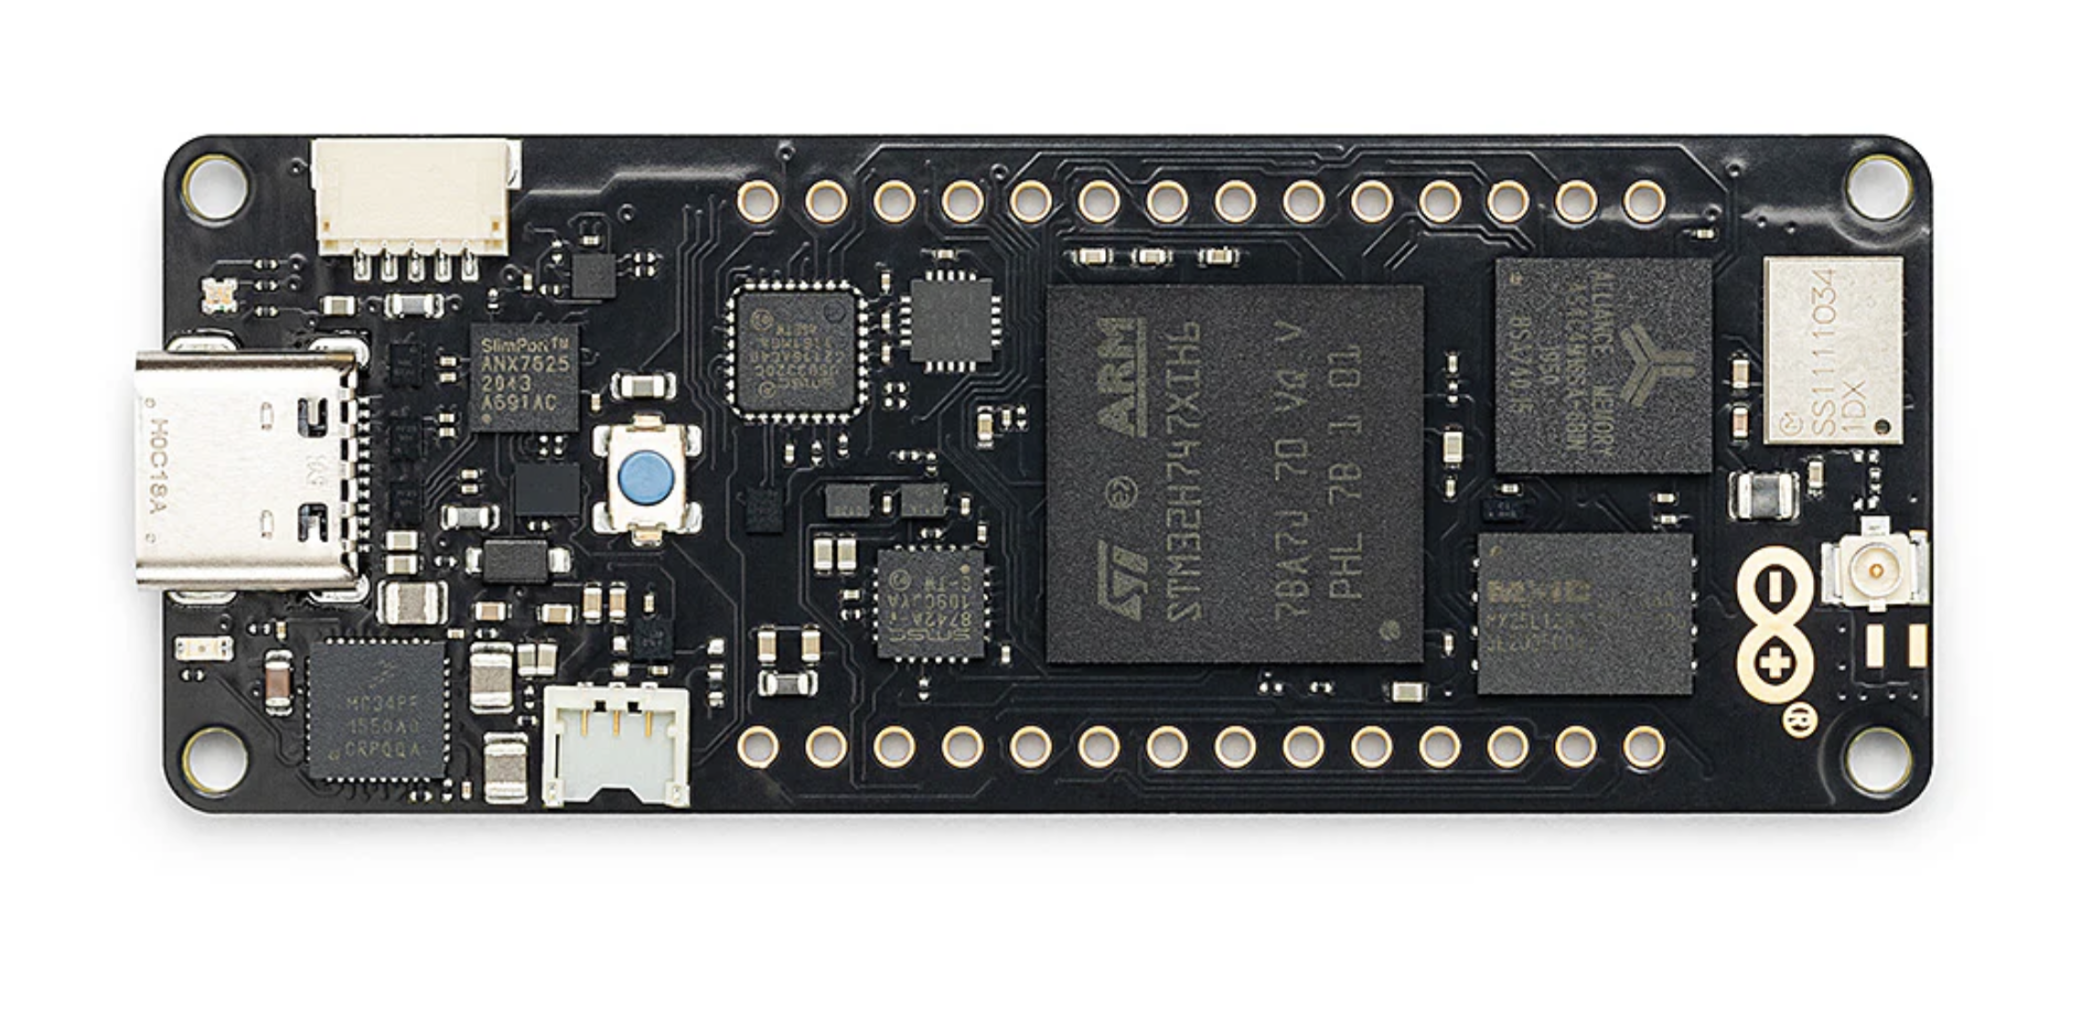
\includegraphics[width=\textwidth]{images/ArduinoPortentaH7.png}
			\vspace{0.2cm}
			\textbf{Figure 1: Arduino PortentaH7}
			
			\column{0.5\textwidth}
			\centering
			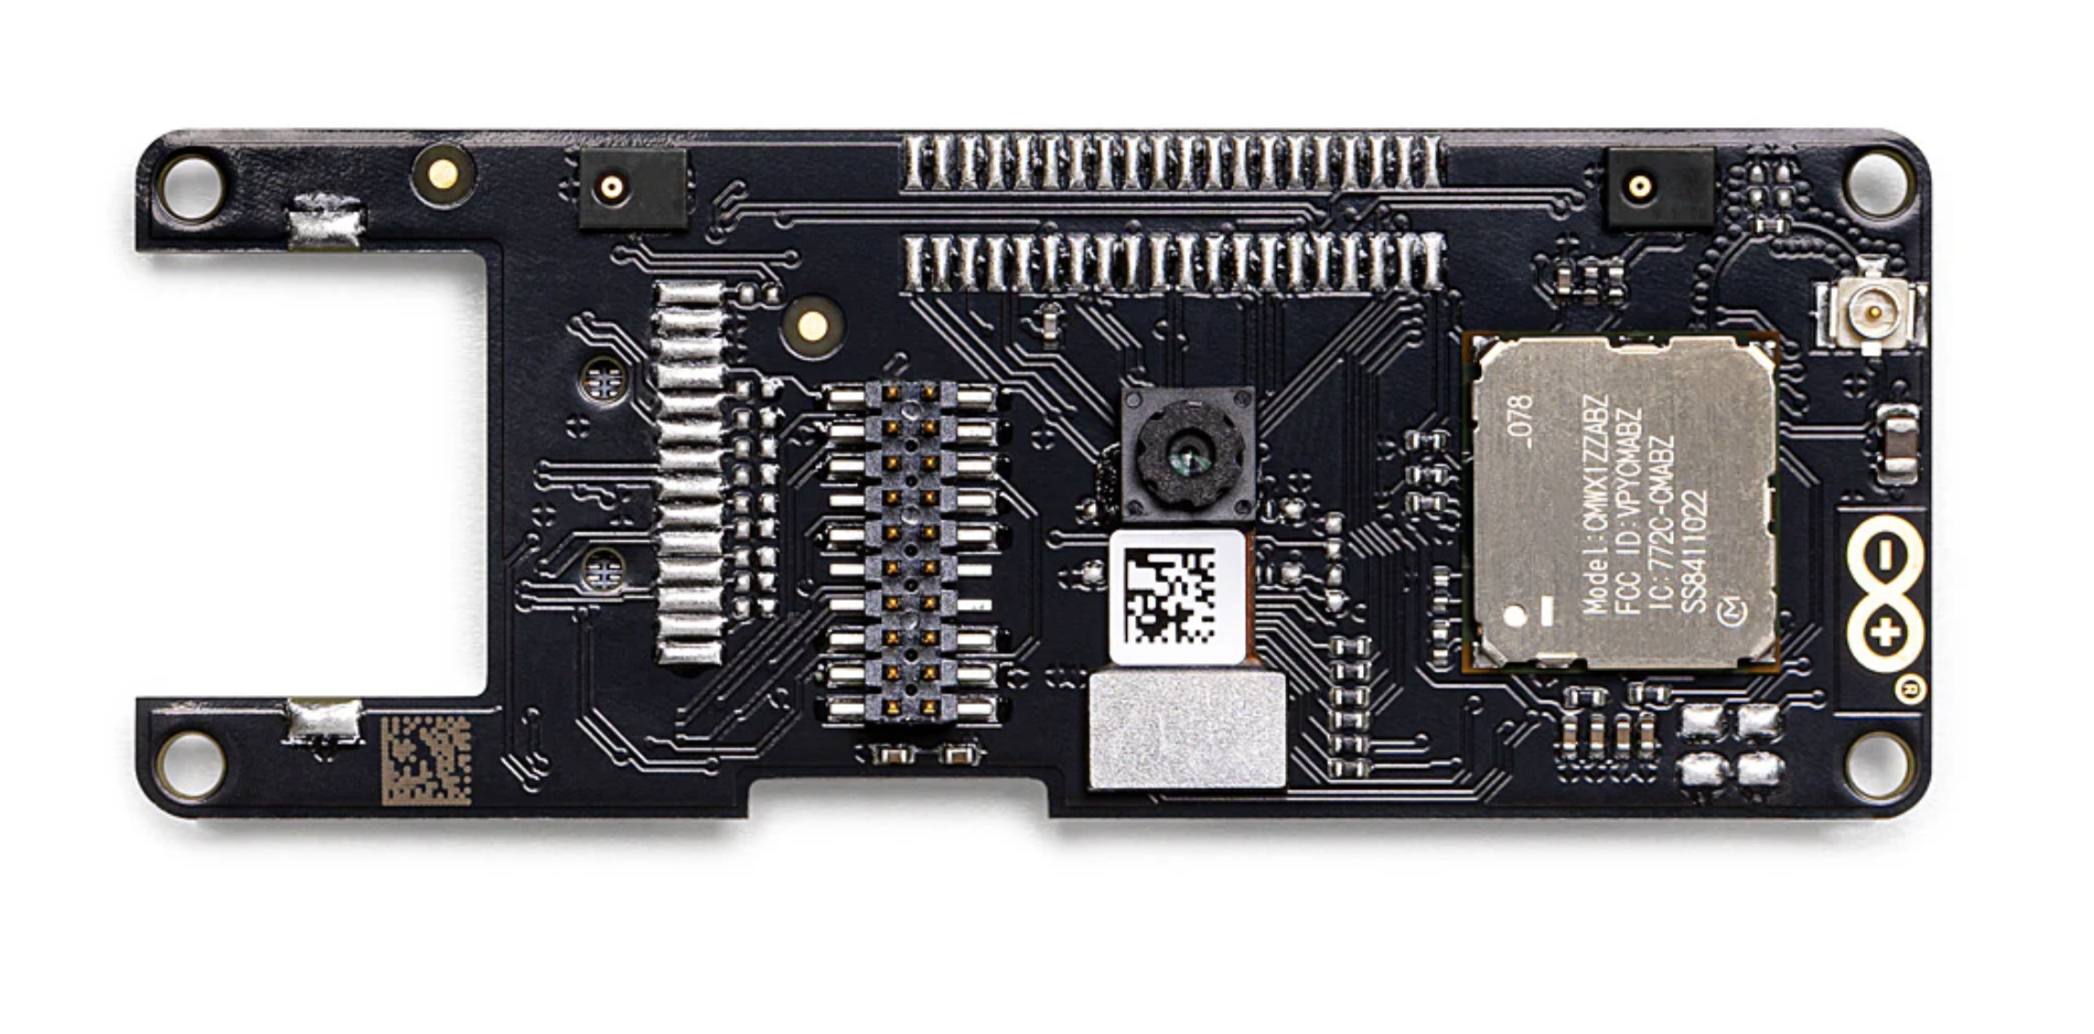
\includegraphics[width=\textwidth]{images/PortentaVisionShield.png}
			\vspace{0.2cm}
			\textbf{Figure 2: PortentaH7 Vision Shield}
		\end{columns}
		
	\end{frame}
	
	\begin{frame}
		\frametitle{1. The Setup:}
		
		\begin{itemize}
			\item {Connect the Portenta Vision Shield to your Portenta H7 as shown in the figure. The top and bottom high density connectors are connected to the corresponding ones on the underside of the H7 board. Plug in the H7 to your computer using the USB-C cable.}
			
				\begin{columns}
					\column{0.5\textwidth}
					\centering
					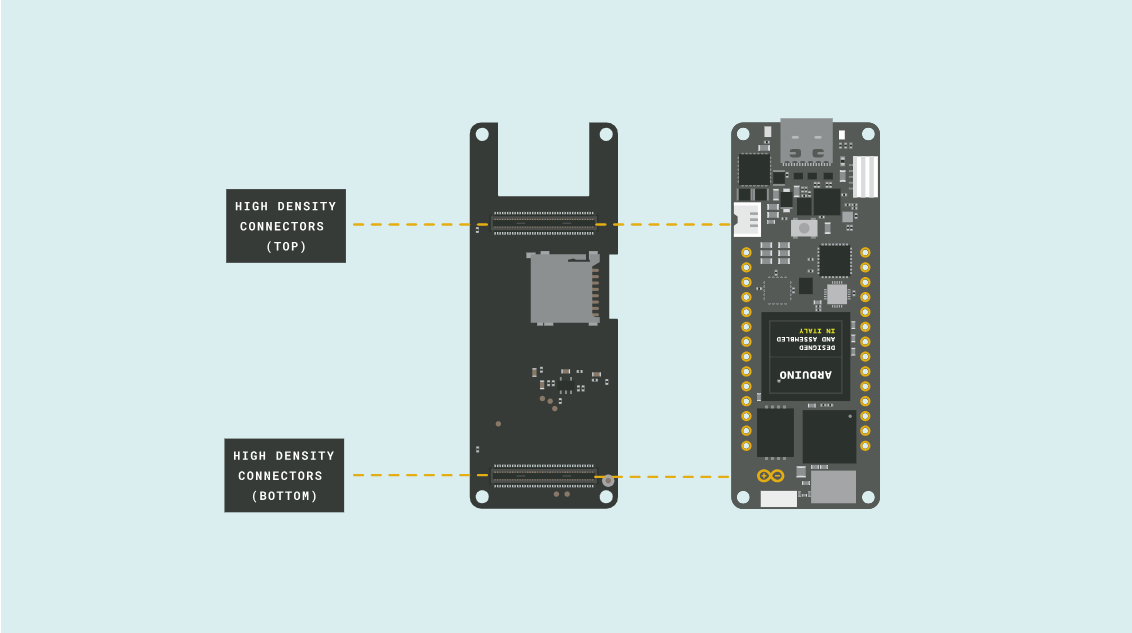
\includegraphics[width=\textwidth]{images/Connection VS.png}
					\vspace{0.2cm}
					\textbf{Figure 3: Connection VS}
				\end{columns}
				
		\end{itemize}
	\end{frame}
	
		\begin{itemize}
			\item \textbf{The Camera:} You will be using the Himax HM-01B0 camera module which has a resolution of 320 by 240 and the output data its in grayscale with 8 bits per pixel (bpp). It is important to have this in mind as the .bmp (bitmap) format has some needed configuration depending on the data being used.
			
			Inside the sketch, you can use these libraries to access the camera APIs
			\begin{verbatim}
			#include "camera.h" // Multi Media Card APIs
			#include "himax.h"  // API to read from the Himax camera found on the Portenta Vision Shield
			\end{verbatim}			
				
			\item \textbf{Bitmap File Format:} The bitmap binary file needs to contain some information in order to tell the computer for example the resolution of the picture and the bit-depth (bpp). Bit depth refers to the color information stored in the image. The higher the bit depth of an image, the more colors it can store. As the bit depth increases, the file size of the image also increases, because more color information has to be stored for each pixel in the image.
				
			The following table shows all the headers, the size of its buffer, offsets, the settings that are being used with their details:
			\begin{table}[h!]
				\centering
				\begin{tabular}{|l|c|l|}
					\hline
					\textbf{Name} & \textbf{Size} & \textbf{Details} \\
					\hline
					Device Independent Bitmap(DIB) & 14 Bytes & Bitmap information, setting the size of the file. \\
					\hline
					File Header & 40 Bytes & This header requires the resolution and the bpp. \\
					\hline
					Palette (Color Map) & 1025 Bytes & This header is mandatory on bitmaps with a bpp greater then 8, setting the grayscale. \\
					\hline
					Image data & 76800 Bytes & The raw image data, in this case, each pixel has 8 bits (1 Byte) and the resolution is 320 x 240, with no compression. \\
					\hline
				\end{tabular}
				\caption{Bitmap File Format Details}
			\end{table}
			
		\end{itemize}	
	
	\begin{frame}
		\frametitle{2. The Sketch}
			You can find the sketch on the latest version of the Arduino-Pro-Tutorials at
			examples > Vision Shield to SD Card bmp > visionShieldBitmap.ino
				\begin{block}{}
					Create a new Arduino sketch called CameraCapture.ino.\newline
					
					To capture the frames you will need to use the functions contained in \textbf{camera.h} which comes with the Portenta core. This library contains all APIs related to frame capturing, motion detection and pattern recognition. Include the header file in your sketch.
					content...
					
						\begin{columns}
							\column{0.5\textwidth}
							\centering
							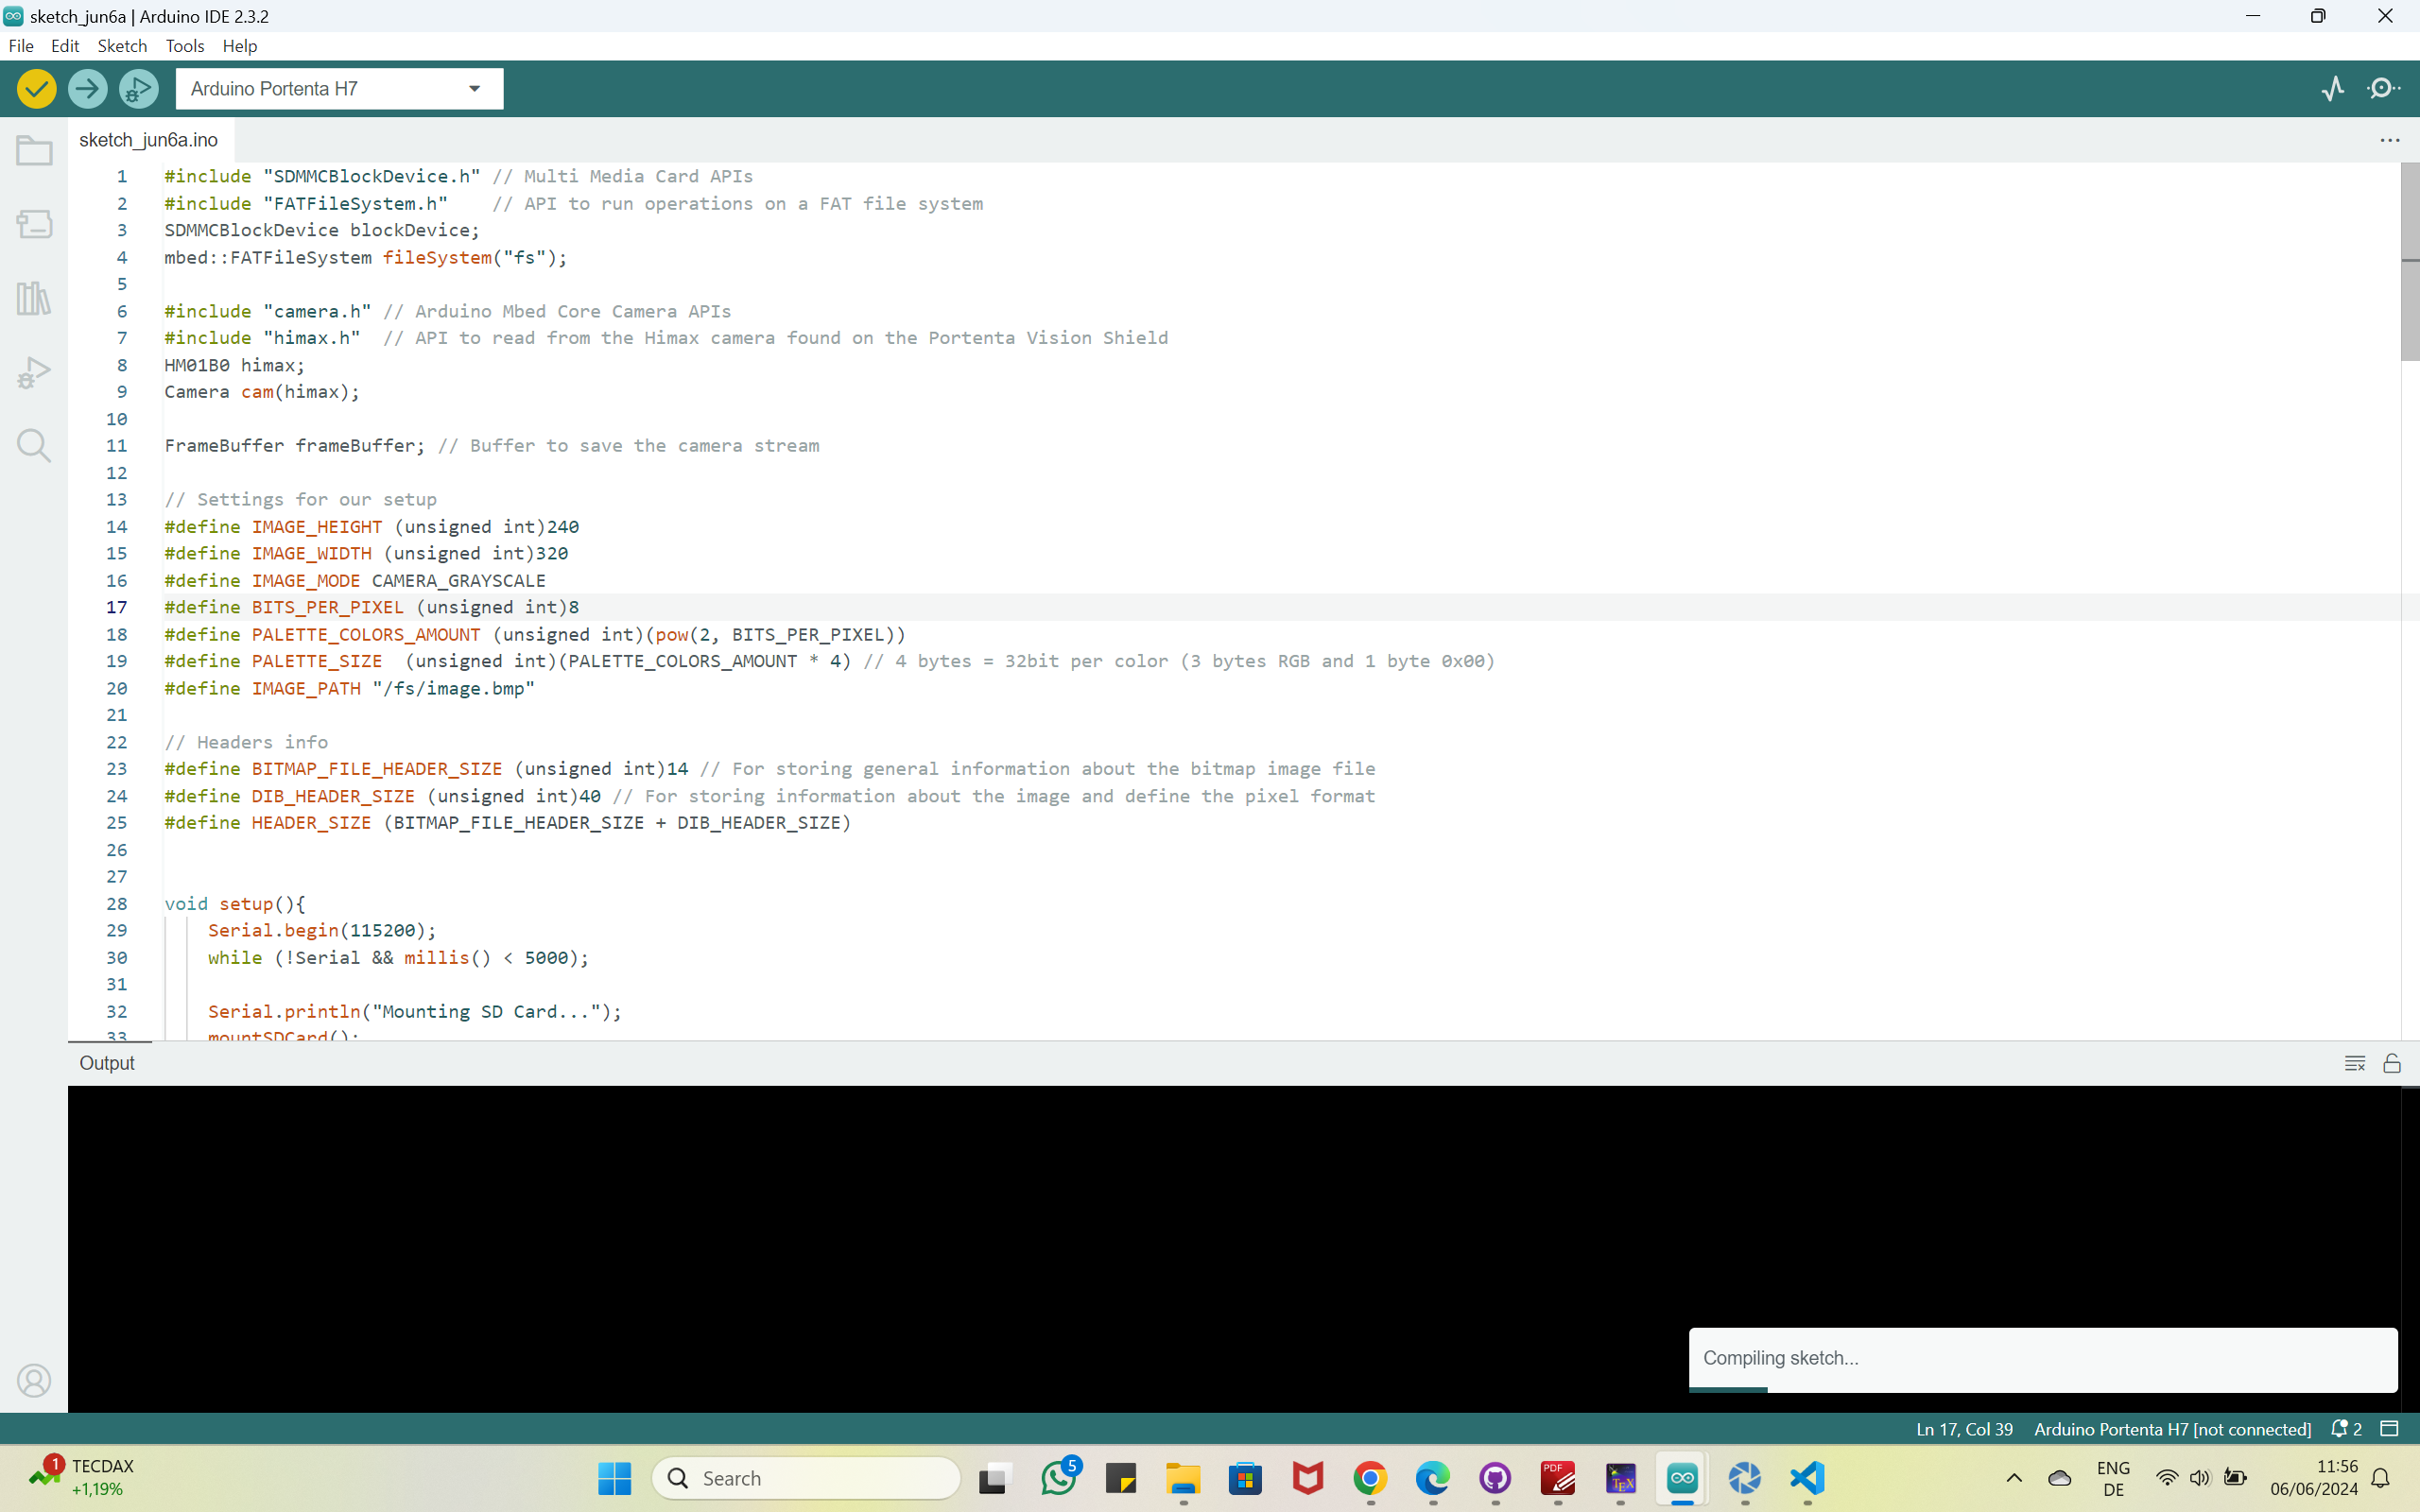
\includegraphics[width=\textwidth]{images/Camera-save.png}
							\vspace{0.2cm}
							\textbf{Figure 4: Camera-save}
						\end{columns}
				\end{block}
			
	\end{frame}
	
	\begin{frame}
		\frametitle{Detailed Explanation of header files}
			\begin{block}{camera.h }
				
				\begin{itemize}
					\item \textbf{Functionality:}Provides an interface to work with camera modules in the Arduino environment. It abstracts the camera hardware specifics and offers functions to initialize the camera, capture images, and configure camera settings.
					\item \textbf{Key Functions: }
					1. begin(resolution, mode, fps): Initializes the camera with specified resolution, image mode (e.g., grayscale), and frames per second. 
					
					2. grabFrame(buffer, timeout): Captures an image frame and stores it in the provided buffer. 
					
					3. getResolution(), setResolution(), etc.: Functions to get and set camera parameters. 
				\end{itemize}
			\end{block}
		
	\end{frame}
	
	\begin{frame}
		\frametitle{}
		\begin{block}{himax.h }
			
			\begin{itemize}
				\item \textbf{Functionality:}Contains specific functions and definitions for working with the Himax HM01B0 camera. This file includes lower-level commands tailored to the Himax camera module, managing settings like exposure, gain, and capturing images.
				\item \textbf{Key Functions: }
				1. init(): Initializes the Himax camera module.  
				
				2. readFrame(buffer): Reads an image frame from the Himax camera and stores it in the provided buffer. 
				
				3. setExposure(time), setGain(value), etc.: Functions to adjust camera settings specific to the Himax HM01B0 module. 
			\end{itemize}
		\end{block}
		
	\end{frame}
	
	\begin{frame}[fragile]
		\frametitle{Capture-save.ino}
		\begin{lstlisting}
			#include "SDMMCBlockDevice.h" // Multi Media Card APIs
			#include "FATFileSystem.h"    // API to run operations on a FAT file system
			SDMMCBlockDevice blockDevice;
			mbed::FATFileSystem fileSystem("fs");
			
			#include "camera.h" // Arduino Mbed Core Camera APIs
			#include "himax.h"  // API to read from the Himax camera found on the Portenta Vision Shield
			HM01B0 himax;
			Camera cam(himax);
			
			FrameBuffer frameBuffer; // Buffer to save the camera stream
			
			// Settings for our setup
			#define IMAGE_HEIGHT (unsigned int)240
			#define IMAGE_WIDTH (unsigned int)320
			#define IMAGE_MODE CAMERA_GRAYSCALE
			#define BITS_PER_PIXEL (unsigned int)8
			#define PALETTE_COLORS_AMOUNT (unsigned int)(pow(2, BITS_PER_PIXEL))
			#define PALETTE_SIZE  (unsigned int)(PALETTE_COLORS_AMOUNT * 4) // 4 bytes = 32bit per color (3 bytes RGB and 1 byte 0x00)
			#define IMAGE_PATH "/fs/image.bmp"
			
			// Headers info
			#define BITMAP_FILE_HEADER_SIZE (unsigned int)14 // For storing general information about the bitmap image file
			#define DIB_HEADER_SIZE (unsigned int)40 // For storing information about the image and define the pixel format
			#define HEADER_SIZE (BITMAP_FILE_HEADER_SIZE + DIB_HEADER_SIZE)
			
			
			void setup(){
				Serial.begin(115200);
				while (!Serial && millis() < 5000);
				
				Serial.println("Mounting SD Card...");
				mountSDCard();
				Serial.println("SD Card mounted.");
				
				// Init the cam QVGA, 30FPS, Grayscale
				if (!cam.begin(CAMERA_R320x240, IMAGE_MODE, 30)){
					Serial.println("Unable to find the camera");
				}
				countDownBlink();
				Serial.println("Fetching camera image...");
				unsigned char *imageData = captureImage();
				digitalWrite(LEDB, HIGH);
				
				Serial.println("Saving image to SD card...");
				saveImage(imageData, IMAGE_PATH);
				
				fileSystem.unmount();
				Serial.println("Done. You can now remove the SD card.");
			}
			
			void loop(){
			}
			
			// Mount File system block
			void mountSDCard(){
				int error = fileSystem.mount(&blockDevice);
				if (error){
					Serial.println("Trying to reformat...");
					int formattingError = fileSystem.reformat(&blockDevice);
					if (formattingError) {            
						Serial.println("No SD Card found");
						while (1);
					}
				}
			}
			
			// Get the raw image data (8bpp grayscale)
			unsigned char * captureImage(){
				if (cam.grabFrame(frameBuffer, 3000) == 0){
					return frameBuffer.getBuffer();
				} else {
					Serial.println("could not grab the frame");
					while (1);
				}
			}
			
			// Set the headers data
			void setFileHeaders(unsigned char *bitmapFileHeader, unsigned char *bitmapDIBHeader, int fileSize){
				// Set the headers to 0
				memset(bitmapFileHeader, (unsigned char)(0), BITMAP_FILE_HEADER_SIZE);
				memset(bitmapDIBHeader, (unsigned char)(0), DIB_HEADER_SIZE);
				
				// File header
				bitmapFileHeader[0] = 'B';
				bitmapFileHeader[1] = 'M';
				bitmapFileHeader[2] = (unsigned char)(fileSize);
				bitmapFileHeader[3] = (unsigned char)(fileSize >> 8);
				bitmapFileHeader[4] = (unsigned char)(fileSize >> 16);
				bitmapFileHeader[5] = (unsigned char)(fileSize >> 24);
				bitmapFileHeader[10] = (unsigned char)HEADER_SIZE + PALETTE_SIZE;
				
				// Info header
				bitmapDIBHeader[0] = (unsigned char)(DIB_HEADER_SIZE);
				bitmapDIBHeader[4] = (unsigned char)(IMAGE_WIDTH);
				bitmapDIBHeader[5] = (unsigned char)(IMAGE_WIDTH >> 8);
				bitmapDIBHeader[8] = (unsigned char)(IMAGE_HEIGHT);
				bitmapDIBHeader[9] = (unsigned char)(IMAGE_HEIGHT >> 8);
				bitmapDIBHeader[14] = (unsigned char)(BITS_PER_PIXEL);
			}
			
			void setColorMap(unsigned char *colorMap){
				//Init the palette with zeroes
				memset(colorMap, (unsigned char)(0), PALETTE_SIZE);
				
				// Gray scale color palette, 4 bytes per color (R, G, B, 0x00)
				for (int i = 0; i < PALETTE_COLORS_AMOUNT; i++) {
					colorMap[i * 4] = i;
					colorMap[i * 4 + 1] = i;
					colorMap[i * 4 + 2] = i;
				}
			}
			
			// Save the headers and the image data into the .bmp file
			void saveImage(unsigned char *imageData, const char* imagePath){
				int fileSize = BITMAP_FILE_HEADER_SIZE + DIB_HEADER_SIZE + IMAGE_WIDTH * IMAGE_HEIGHT;
				FILE *file = fopen(imagePath, "w");
				
				// Bitmap structure (Head + DIB Head + ColorMap + binary image)
				unsigned char bitmapFileHeader[BITMAP_FILE_HEADER_SIZE];
				unsigned char bitmapDIBHeader[DIB_HEADER_SIZE];
				unsigned char colorMap[PALETTE_SIZE]; // Needed for <= 8bpp grayscale bitmaps    
				
				setFileHeaders(bitmapFileHeader, bitmapDIBHeader, fileSize);
				setColorMap(colorMap);
				
				// Write the bitmap file
				fwrite(bitmapFileHeader, 1, BITMAP_FILE_HEADER_SIZE, file);
				fwrite(bitmapDIBHeader, 1, DIB_HEADER_SIZE, file);
				fwrite(colorMap, 1, PALETTE_SIZE, file);
				fwrite(imageData, 1, IMAGE_HEIGHT * IMAGE_WIDTH, file);
				
				// Close the file stream
				fclose(file);
			}
			
			void countDownBlink(){
				for (int i = 0; i < 6; i++){
					digitalWrite(LEDG, i % 2);
					delay(500);
				}
				digitalWrite(LEDG, HIGH);
				digitalWrite(LEDB, LOW);
			}   
					
		\end{lstlisting}
	\end{frame}
		
	\begin{frame}[fragile]
		\frametitle{Continue...}
		\begin{lstlisting}
			// Write the bitmap file
			fwrite(bitmapFileHeader, 1, BITMAP_FILE_HEADER_SIZE, file);
			fwrite(bitmapDIBHeader, 1, DIB_HEADER_SIZE, file);
			fwrite(colorMap, 1, PALETTE_SIZE, file);
			fwrite(imageData, 1, IMAGE_HEIGHT * IMAGE_WIDTH, file);
			
			// Close the file stream
			fclose(file);
			}
			
			void countDownBlink(){
			for (int i = 0; i < 6; i++){
				digitalWrite(LEDG, i % 2);
				delay(500);
			}
			digitalWrite(LEDG, HIGH);
			digitalWrite(LEDB, LOW);
			} 
		\end{lstlisting}
	\end{frame}
	
	\begin{frame}		
		\frametitle{Upload the Sketch}
		\framesubtitle{Saving on SD Card:}
			\begin{itemize}
				\item Select the right serial port on your IDE and upload the Arduino sketch to your Portenta H7.
				\item Insert a micro SD Card into the Portenta Vision Shield.
				\item Connect the Portenta Vision Shield to the Portenta H7.
				\item Once the sketch is uploaded, open the Serial Monitor or wait 5 seconds: you should see that everything is fine and the capture has been taken.
				\item Once the capture is saved, remove the SD Card and plug it into a computer/phone with an SD Card reader, open the storage unit, look for a bitmap called image.bmp and open it to check the result. You will be able to see a grayscale image on your device's image viewer. \newpage
			\end{itemize}
			
				\begin{columns}
					\column{0.5\textwidth}
					\centering
					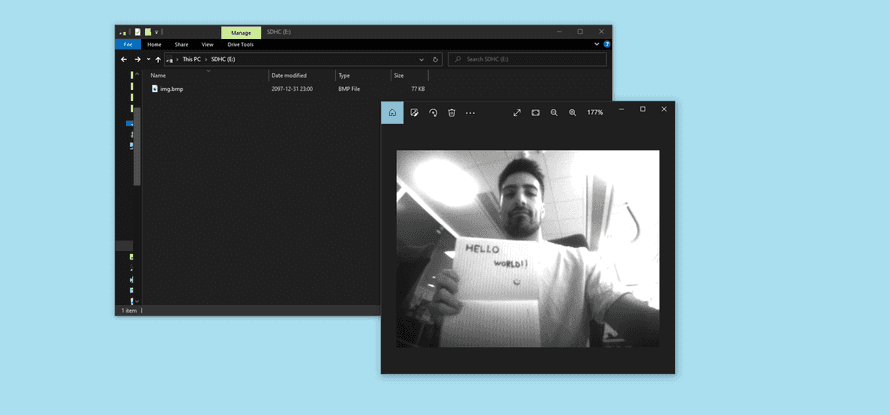
\includegraphics[width=\textwidth]{images/output-view.png}
					\vspace{0.2cm}
					\textbf{Figure 5: output-view}
				\end{columns}

	\end{frame}
	
	\begin{frame}		
		\frametitle{Saving on PC:}
		\framesubtitle{Steps to Save the Image on Your PC:}
		\begin{itemize}
			\item 1. Modify Your Arduino Code:
			\item 2. Set Up Serial Communication on Your PC:\newline
				a. Use a serial terminal application like PuTTY, CoolTerm, or the built-in Serial Monitor in the Arduino IDE.\newline
				b .Ensure the serial terminal is set to the correct baud rate (115200 in this case) and connected to the correct serial port.
			\item 3. Receive and Save the Data on Your PC:\newline
				a. Open the serial terminal and start the Arduino sketch. The image data will be sent over the serial connection.\newline
				b. You will need a script or a tool on your PC to capture the incoming serial data and save it to a BMP file.
			\item Once the sketch is uploaded, open the Serial Monitor or wait 5 seconds: you should see that everything is fine and the capture has been taken.
			\item Once the capture is saved, remove the SD Card and plug it into a computer/phone with an SD Card reader, open the storage unit, look for a bitmap called image.bmp and open it to check the result. You will be able to see a grayscale image on your device's image viewer. \newpage
		\end{itemize}
		
	\end{frame}
	
	\begin{frame}[fragile]
		\frametitle{Python Script to Receive and Save Image Data on PC:}
		\begin{lstlisting}
			import serial
			
			# Constants from Arduino code
			BITMAP_FILE_HEADER_SIZE = 14
			DIB_HEADER_SIZE = 40
			IMAGE_WIDTH = 320
			IMAGE_HEIGHT = 240
			PALETTE_COLORS_AMOUNT = 256
			PALETTE_SIZE = PALETTE_COLORS_AMOUNT * 4
			
			def receive_image(serial_port, file_path):
			ser = serial.Serial(serial_port, 115200, timeout=10)
			file_size = BITMAP_FILE_HEADER_SIZE + DIB_HEADER_SIZE + IMAGE_WIDTH * IMAGE_HEIGHT + PALETTE_SIZE
			
			# Read the entire file
			image_data = ser.read(file_size)
			
			with open(file_path, 'wb') as file:
			file.write(image_data)
			
			ser.close()
			
			if __name__ == "__main__":
			serial_port = "COM3"  # Replace with your serial port (e.g., /dev/ttyUSB0 for Linux)
			file_path = "image.bmp"  # Path where you want to save the image
			
			receive_image(serial_port, file_path)
			print("Image received and saved as", file_path)
			
			 
	\end{lstlisting}
	\end{frame}
	
	\section{Conclusion}
	\begin{frame}
		\frametitle{Conclusion}
		In this presentation you learned how to capture frames with your Portenta Vision Shield's Camera in the Arduino IDE, encode it with the bitmap standards and save it to an SD Card and PC.
		
	\end{frame}
	
	\section{Future Work}
	\begin{frame}
		\frametitle{Future Work}
		\begin{itemize}
			\item Creating a Basic Face Filter With OpenMV
			\item Connecting the Portenta Vision Shield to The Things Network(TTN) Using LoRa 
			\item Send the camera data through it LoRa.
		\end{itemize}
	\end{frame}
	
	\STANDARD{}
{
  \begin{columns}
    \begin{column}{0.35\textwidth}
      \begin{block}{~~~~~~Thank you}
        \centering
        for your attention
      \end{block}
    \end{column}
  \end{columns}
}

\MYNOTE{Ja, \textbf{Vielen} Dank, für Ihre Aufmerksamkeit}


	
\end{document}
